\documentclass[12pt]{article}
\usepackage{graphicx}
\usepackage{float}
\title{Preliminary Analysis of Actual Data II}

\begin{document}
\maketitle

\section{Description of Work Done}
\begin{enumerate}
\item Create training and test sets. Holdout 63 conditions across genes and use 251 conditions for training.
\item Set number of reps to be the 100*(prior probability) rounded to next highest 10. Set to 1 if prior probability is 0. Creates 1-10 reps. (most TFs get 1 rep.).
\item For illustration, chose 100 genes and ran BART. Used 1000 burn-in, 2000 posterior. Tried for ntree=5 and 10. Should add 20. 
\item 100 Bootstrap Iterations where extra columns are random TFs and $\mathbf{y}$ is permuted to break all dependencies. 
\item Considered selection for $95^{th}$ quantile using simultaneous coverage and point-wise coverage. FDR is probably better.  
\end{enumerate}

\newpage
\section{Inclusions}
\subsection*{Pointwise}
\begin{itemize}
\item 474 genes for 5 trees.
\item 506 genes for 10 trees.
\end{itemize}
Is this sensible or counter-intuitive? Seems sensible since 5 may be bottle-necking too hard.


\subsection*{Simultaneous}
\begin{itemize}
\item 35 for 5 trees.
\item 52 for 10 trees. 
\end{itemize}
Perhaps too stringent. Really want .05 simultaneous coverage? FDR.



\section{Correlation Histograms}
\subsection*{Between Model Correlation}
\begin{figure}[H]
\centerline{\includegraphics[scale=.6]{corList.pdf}}
\caption{\it Correlations of inclusion frequencies for 5 and 10 tree models}
\label{fig:version1}  
\end{figure}

\section*{Within Model Correlations}
These are correlations between prior PROBABILITIES, not columns and TF inclusion frequency. 
\begin{figure}[H]
\centerline{\includegraphics[scale=.6]{inclTFcor.pdf}}
\caption{\it Correlations between inclusion frequencies and prior probability.}
\label{fig:version1}  
\end{figure}
In above plot, notice that correlation goes up as number of trees goes up.
\begin{verbatim}
> summary(cor10,na.rm=T)
    Min.  1st Qu.   Median     Mean  3rd Qu.     Max. 
-0.15880 -0.04497  0.14450  0.21450  0.47160  0.76410 
    NA's 
       3 
> summary(cor5,na.rm=T)
    Min.  1st Qu.   Median     Mean  3rd Qu.     Max. 
-0.16440 -0.05901  0.09428  0.12570  0.22480  0.74620 
    NA's 
       3 
\end{verbatim}



\section{Likelihood vs. Prior Correlation Plots }

\begin{figure}[H]
\centerline{\includegraphics[scale=.6]{shanePrior.pdf}}
\caption{\it Plots of correlations between correlation of gene and TF expression vs. correlations inclusion frequency and prior probability and inclusion frequency}
\label{fig:version1}  
\end{figure}


Due to the NAs, second plot removes any point that had a uniform prior in BART. Interesting to compare and see that the prior has more weight in this case. Sensible since these are the models where prior mattered more. 
\begin{figure}[H]
\centerline{\includegraphics[scale=.6]{shaneWeights.pdf}}
\caption{\it Plots of correlations between correlation of gene and TF expression vs. correlations inclusion frequency and prior weights and inclusion frequency}
\label{fig:version2}  
\end{figure}



\section{Sample Histograms of Null Distributions}

\begin{figure}[H]
\centerline{\includegraphics[scale=.70]{null5.pdf}}
\caption{\it Null Distributions for first 9 TFs for gene YAL001C (using ORF) in 5 tree model.}
\label{fig:version2}  
\end{figure}

\begin{figure}[H]
\centerline{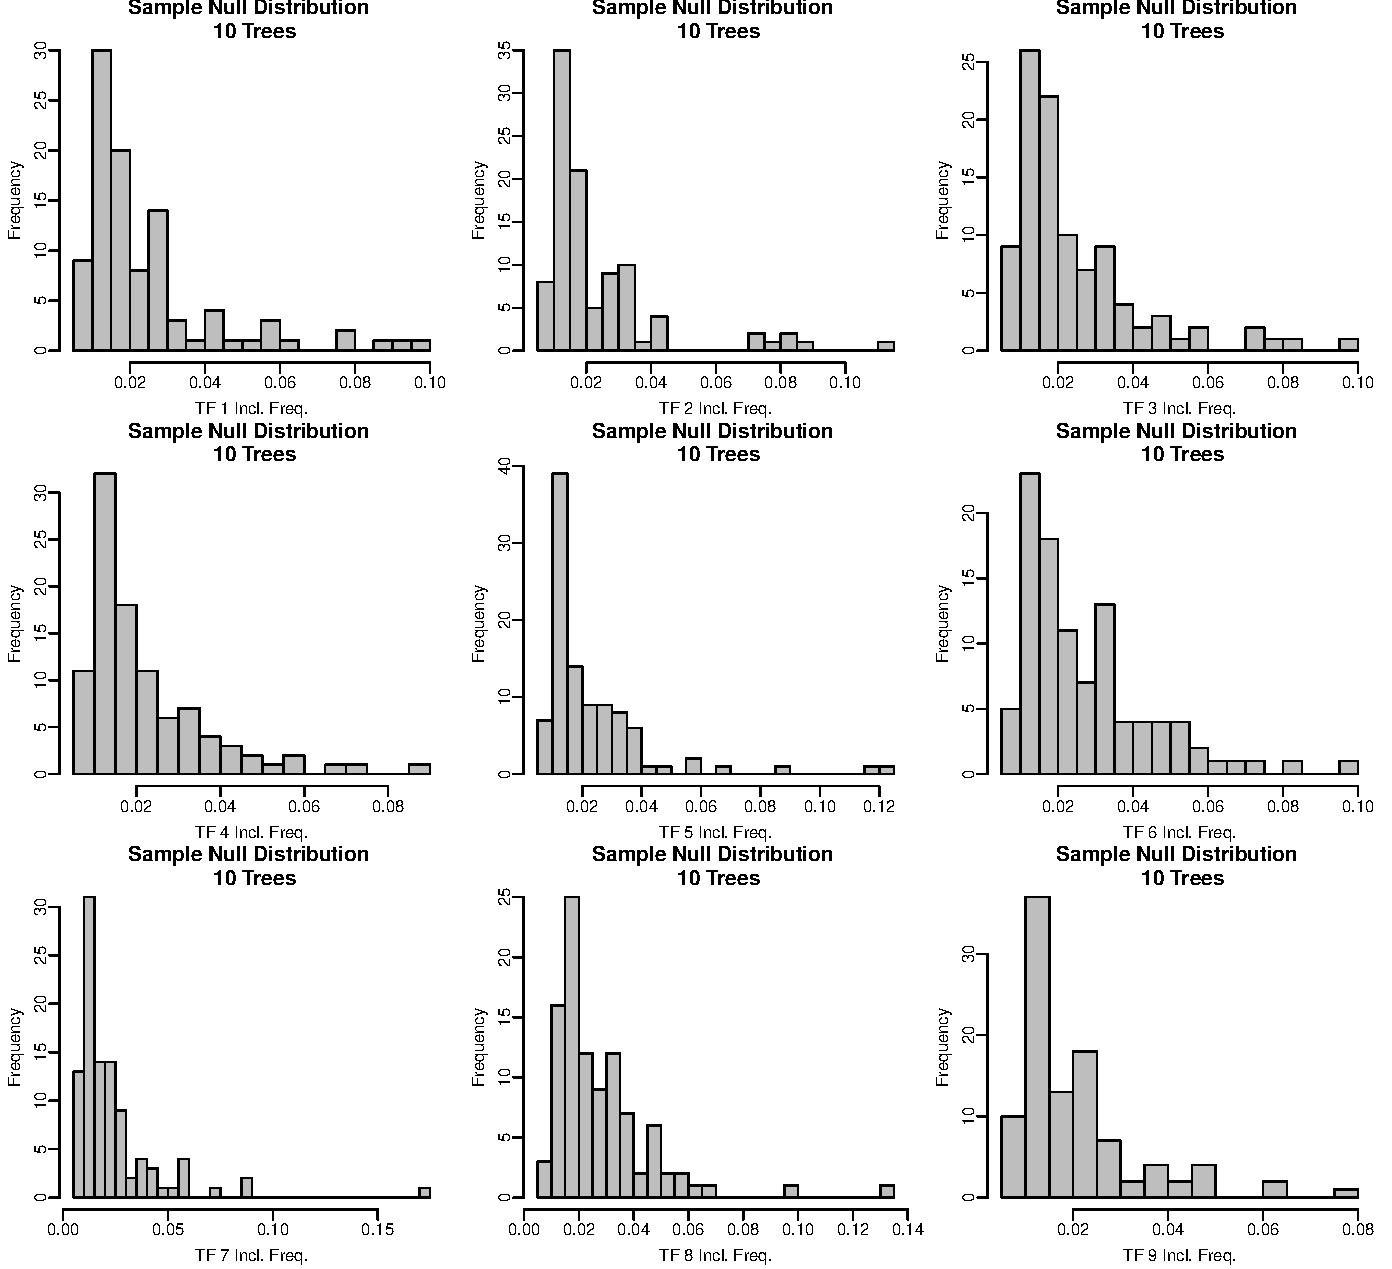
\includegraphics[scale=.7]{null10.pdf}}
\caption{\it Null Distributions for first 9 TFs for gene YAL001C (using ORF) in 10 tree model.}\label{fig:version2}  
\end{figure}


\end{document}